% diag_handshake: TikZ twin of paper/figures/diag_handshake.pdf (generated by diag_common.py).
% Coordinates are inches (y up). Needs \usepackage{tikz}. Body font 7 pt.
\definecolor{dgA}{HTML}{F0F0F0}\definecolor{dgB}{HTML}{DCDCDC}\definecolor{dgC}{HTML}{C4C4C4}
\definecolor{dgAtk}{HTML}{F2C9B8}\definecolor{dgHw}{HTML}{E3EEF7}
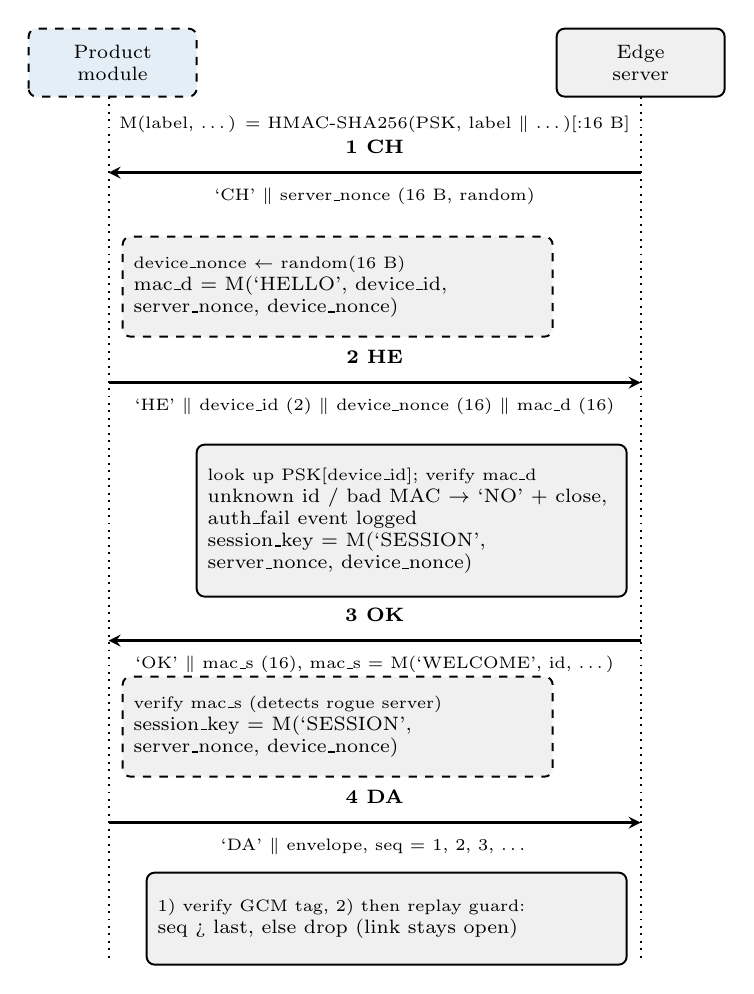
\begin{tikzpicture}[x=1in,y=1in,>=stealth,font=\fontsize{7}{8}\selectfont,line width=0.7pt]
\draw[rounded corners=2.9pt,fill=dgHw,line width=0.7pt,dashed] (0.020,4.380) rectangle (0.860,4.720);
\node[align=center,inner sep=0pt] at (0.440,4.550) {\fontsize{6.8}{7.6}\selectfont Product\\ module};
\draw[rounded corners=2.9pt,fill=dgA,line width=0.7pt] (2.660,4.380) rectangle (3.500,4.720);
\node[align=center,inner sep=0pt] at (3.080,4.550) {\fontsize{6.8}{7.6}\selectfont Edge\\ server};
\draw[line width=0.7pt,dotted] (0.420,4.380) -- (0.420,0.050);
\draw[line width=0.7pt,dotted] (3.080,4.380) -- (3.080,0.050);
\node[align=center,fill=white,inner sep=1pt] at (1.750,4.240) {\fontsize{6.5}{7.3}\selectfont M(label, …) = HMAC-SHA256(PSK, label $\Vert$ …)[:16 B]};
\draw[->,line width=0.9pt] (3.080,4.000) -- (0.420,4.000);
\node[align=center,inner sep=0pt] at (1.750,4.130) {\bfseries \fontsize{7}{7.8}\selectfont 1  CH};
\node[align=center,inner sep=0pt] at (1.750,3.880) {\fontsize{6.5}{7.3}\selectfont ‘CH’ $\Vert$ server\_nonce (16 B, random)};
\draw[rounded corners=2.9pt,fill=dgA,line width=0.7pt,dashed] (0.490,3.180) rectangle (2.640,3.680);
\node[align=flush left,anchor=west,inner sep=0pt] at (0.540,3.430) {\fontsize{6.5}{7.3}\selectfont device\_nonce $\leftarrow$ random(16 B)\\ mac\_d = M(‘HELLO’, device\_id,\\   server\_nonce, device\_nonce)};
\draw[->,line width=0.9pt] (0.420,2.950) -- (3.080,2.950);
\node[align=center,inner sep=0pt] at (1.750,3.080) {\bfseries \fontsize{7}{7.8}\selectfont 2  HE};
\node[align=center,inner sep=0pt] at (1.750,2.830) {\fontsize{6.5}{7.3}\selectfont ‘HE’ $\Vert$ device\_id (2) $\Vert$ device\_nonce (16) $\Vert$ mac\_d (16)};
\draw[rounded corners=2.9pt,fill=dgA,line width=0.7pt] (0.860,1.880) rectangle (3.010,2.640);
\node[align=flush left,anchor=west,inner sep=0pt] at (0.910,2.260) {\fontsize{6.5}{7.3}\selectfont look up PSK[device\_id]; verify mac\_d\\ unknown id / bad MAC $\rightarrow$ ‘NO’ + close,\\   auth\_fail event logged\\ session\_key = M(‘SESSION’,\\   server\_nonce, device\_nonce)};
\draw[->,line width=0.9pt] (3.080,1.660) -- (0.420,1.660);
\node[align=center,inner sep=0pt] at (1.750,1.790) {\bfseries \fontsize{7}{7.8}\selectfont 3  OK};
\node[align=center,inner sep=0pt] at (1.750,1.540) {\fontsize{6.5}{7.3}\selectfont ‘OK’ $\Vert$ mac\_s (16),  mac\_s = M(‘WELCOME’, id, …)};
\draw[rounded corners=2.9pt,fill=dgA,line width=0.7pt,dashed] (0.490,0.980) rectangle (2.640,1.480);
\node[align=flush left,anchor=west,inner sep=0pt] at (0.540,1.230) {\fontsize{6.5}{7.3}\selectfont verify mac\_s (detects rogue server)\\ session\_key = M(‘SESSION’,\\   server\_nonce, device\_nonce)};
\draw[->,line width=0.9pt] (0.420,0.750) -- (3.080,0.750);
\node[align=center,inner sep=0pt] at (1.750,0.880) {\bfseries \fontsize{7}{7.8}\selectfont 4  DA};
\node[align=center,inner sep=0pt] at (1.750,0.630) {\fontsize{6.5}{7.3}\selectfont ‘DA’ $\Vert$ envelope, seq = 1, 2, 3, …};
\draw[rounded corners=2.9pt,fill=dgA,line width=0.7pt] (0.610,0.040) rectangle (3.010,0.500);
\node[align=flush left,anchor=west,inner sep=0pt] at (0.660,0.270) {\fontsize{6.5}{7.3}\selectfont 1) verify GCM tag, 2) then replay guard:\\ seq > last, else drop (link stays open)};
\end{tikzpicture}
